% ─────────────────────────────────────────────────
% VERSION TRACKER — No modificar este bloque
% Versión:    Tesis Humanizada
% Archivo:    Anexos/AnexoCasosDeUso.tex
% Última mod:  2026-05-08T08:45:26
% Git commit:  cc9c766f @ main
% Audiencia:   general
% Verificar antes de editar: bash check_tesis_version.sh overleaf_tesis_humanizado/Anexos/AnexoCasosDeUso.tex
% ─────────────────────────────────────────────────


\section*{Diagramas UML del sistema} \label{anexoUML}
\addcontentsline{toc}{section}{Diagramas UML del sistema}

A continuación se presentan los diagramas UML que modelan el sistema Pymetory desde distintas perspectivas: casos de uso, secuencia de operaciones, componentes de software y despliegue de infraestructura.

\subsection*{Diagrama de Casos de Uso}

El sistema define dos actores con responsabilidades claramente delimitadas: el Administrador, con acceso completo a todos los módulos, y el Operario, con acceso exclusivo a las funciones de operación diaria.

\begin{figure}[H]
	\centering
	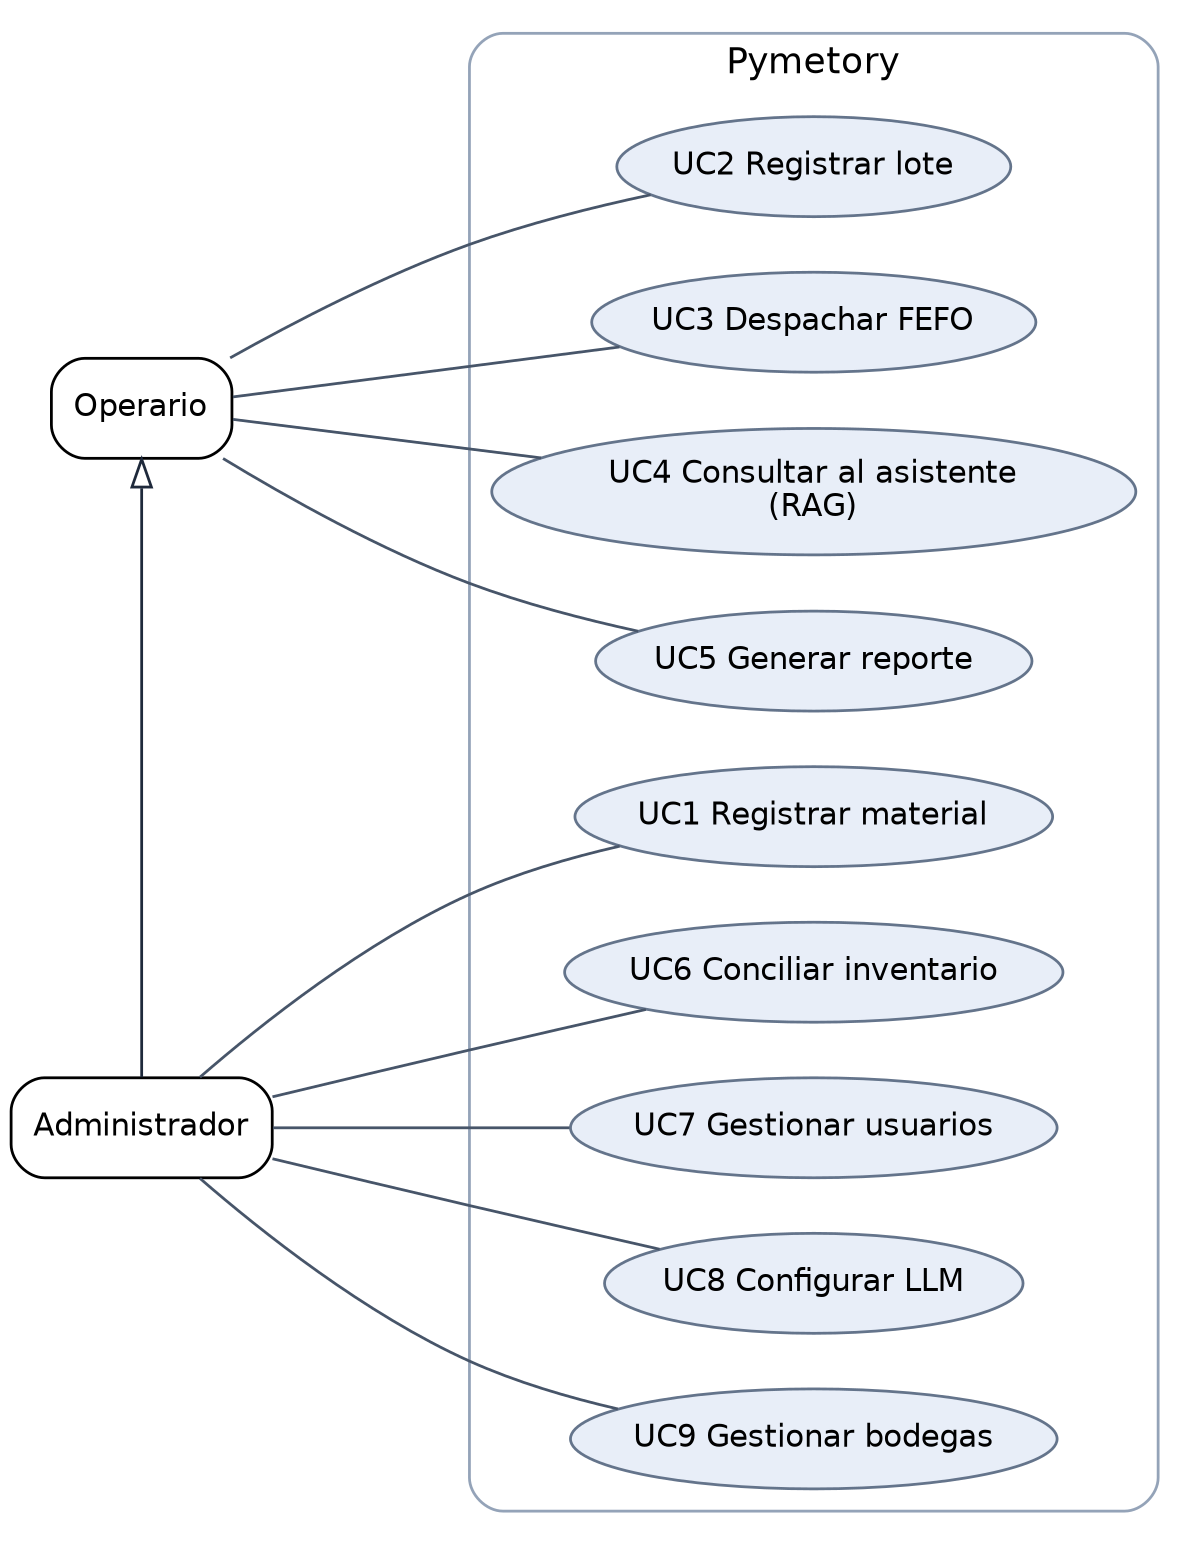
\includegraphics[width=14cm]{Anexos/Imagenes/CasosDeUso.png}
	\caption{Diagrama de casos de uso del sistema Pymetory. El Administrador tiene acceso a los nueve casos de uso; el Operario accede a los cinco casos de uso operativos: Registrar Material, Registrar Lote, Despachar FEFO, Consultar RAG y Gestionar Kanban.}
	\label{fig:casosDeUso}
\end{figure}

Los nueve casos de uso del sistema son:

\begin{enumerate}
	\item \textbf{UC1 — Registrar Material:} El operario o administrador ingresa un nuevo material al catálogo, especificando código único, nombre, unidad de medida y bodega destino. El sistema valida que el código no esté duplicado y crea el registro junto con un lote inicial y su movimiento de entrada en el Kardex.
	\item \textbf{UC2 — Registrar Lote:} Permite ingresar un nuevo lote de un material existente, especificando número de lote, cantidad, costo unitario, fecha de vencimiento y bodega destino. El sistema actualiza el stock y registra el movimiento.
	\item \textbf{UC3 — Despachar FEFO:} El operario solicita una cantidad de material para un motivo específico (producción, venta, desperdicio o ajuste). El sistema selecciona automáticamente los lotes más próximos a vencer y descuenta de ellos hasta cubrir la cantidad solicitada.
	\item \textbf{UC4 — Consultar RAG:} El usuario escribe una pregunta en lenguaje natural sobre el inventario. El sistema clasifica la intención, construye contexto a partir de la base de datos real y envía la consulta al modelo de lenguaje, que responde con datos actualizados del inventario.
	\item \textbf{UC5 — Generar Reporte:} El administrador puede exportar reportes del inventario en formato PDF o CSV, con filtros por bodega y estado del lote. Cada exportación queda registrada en la auditoría.
	\item \textbf{UC6 — Conciliar:} El administrador corrige discrepancias entre el inventario físico y el lógico ingresando la cantidad real verificada en bodega. El sistema registra automáticamente un movimiento de ajuste en el Kardex.
	\item \textbf{UC7 — Gestionar Usuarios:} El administrador registra nuevos usuarios, asigna roles (admin u operario) y gestiona el control de acceso RBAC del sistema.
	\item \textbf{UC8 — Configurar LLM:} El administrador ajusta los parámetros del módulo de inteligencia artificial: modelo a utilizar, temperatura de las respuestas, tokens máximos, fuente (local o externa) y clave de API.
	\item \textbf{UC9 — Gestionar Bodegas:} El administrador crea, edita y monitorea las bodegas del sistema, registrando su capacidad máxima y visualizando el porcentaje de ocupación en tiempo real.
\end{enumerate}

\subsection*{Diagrama de Secuencia — Registro de Entrada}

\begin{figure}[H]
	\centering
	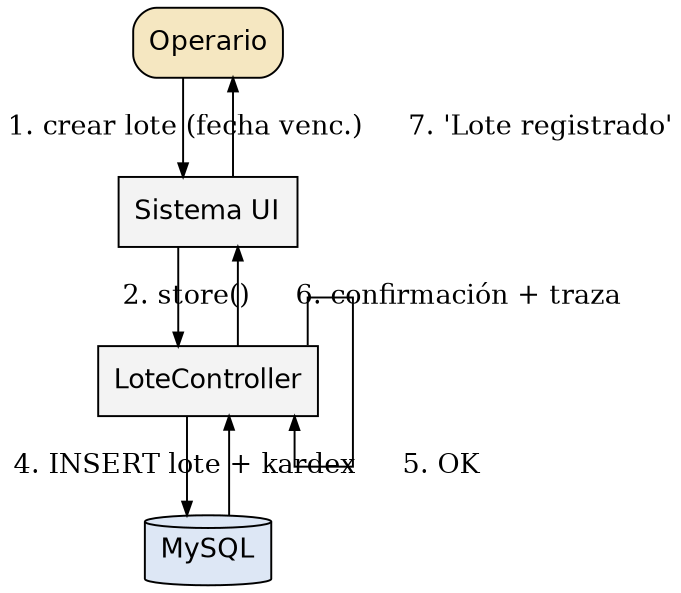
\includegraphics[width=14cm]{Anexos/Imagenes/SecuenciaRegistroEntrada.png}
	\caption{Diagrama de secuencia del registro de entrada de un lote. Muestra la interacción entre el Operario, el frontend React+Inertia.js, el InventoryController y MySQL, incluyendo la transacción atómica que garantiza la creación simultánea del lote y su movimiento de Kardex.}
	\label{fig:secRegistroEntrada}
\end{figure}

\subsection*{Diagrama de Secuencia — Consulta RAG}

\begin{figure}[H]
	\centering
	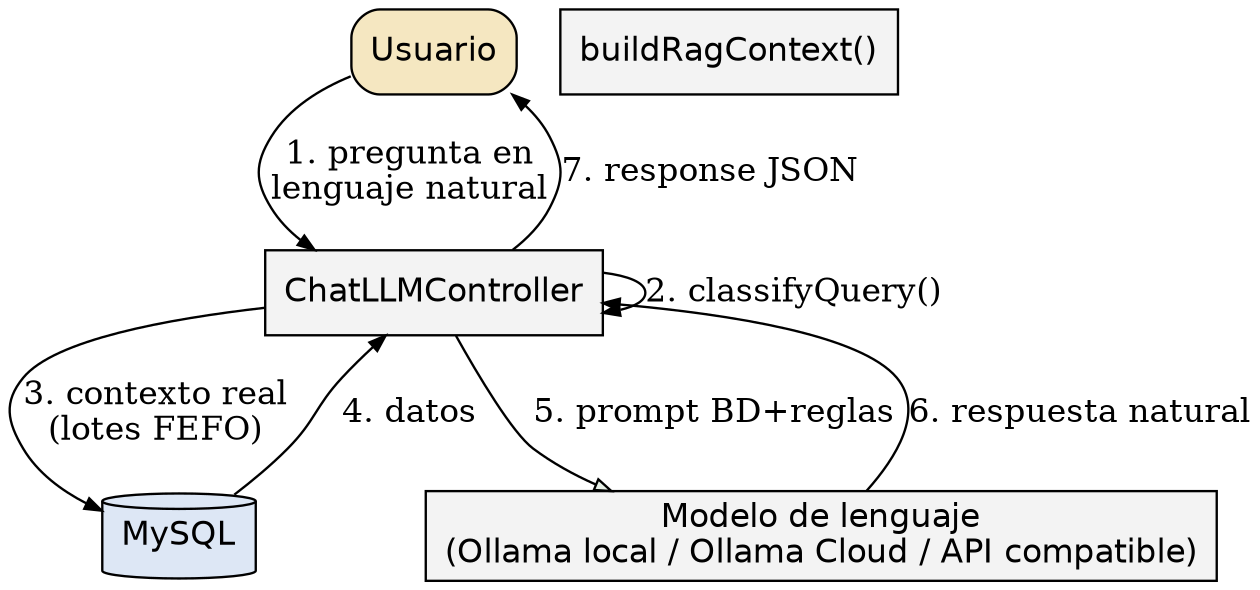
\includegraphics[width=14cm]{Anexos/Imagenes/SecuenciaConsultaRAG.png}
	\caption{Diagrama de secuencia de una consulta al módulo RAG. El flujo muestra la clasificación de intención, la construcción del contexto a partir de la base de datos, el envío del prompt enriquecido al LLM y el almacenamiento de la respuesta en el historial de chat.}
	\label{fig:secConsultaRAG}
\end{figure}

\subsection*{Diagrama de Secuencia — Despacho FEFO}

\begin{figure}[H]
	\centering
	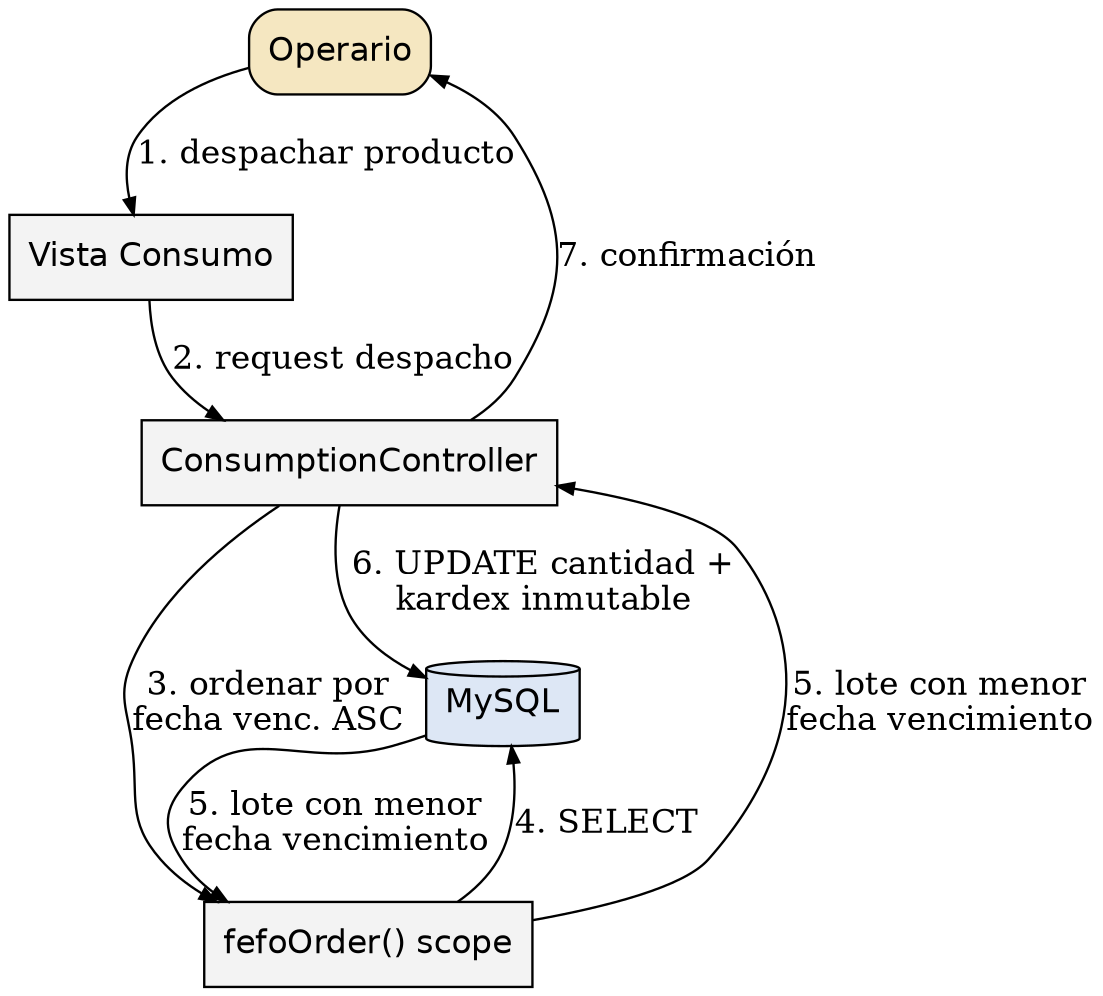
\includegraphics[width=14cm]{Anexos/Imagenes/SecuenciaDespachoFEFO.png}
	\caption{Diagrama de secuencia del despacho aplicando el algoritmo FEFO. Ilustra cómo el sistema ordena los lotes por fecha de vencimiento, descuenta del más próximo primero, marca lotes agotados como \texttt{consumed} y registra cada movimiento en el Kardex inmutable dentro de una transacción atómica.}
	\label{fig:secDespachoFEFO}
\end{figure}

\subsection*{Diagrama de Componentes}

\begin{figure}[H]
	\centering
	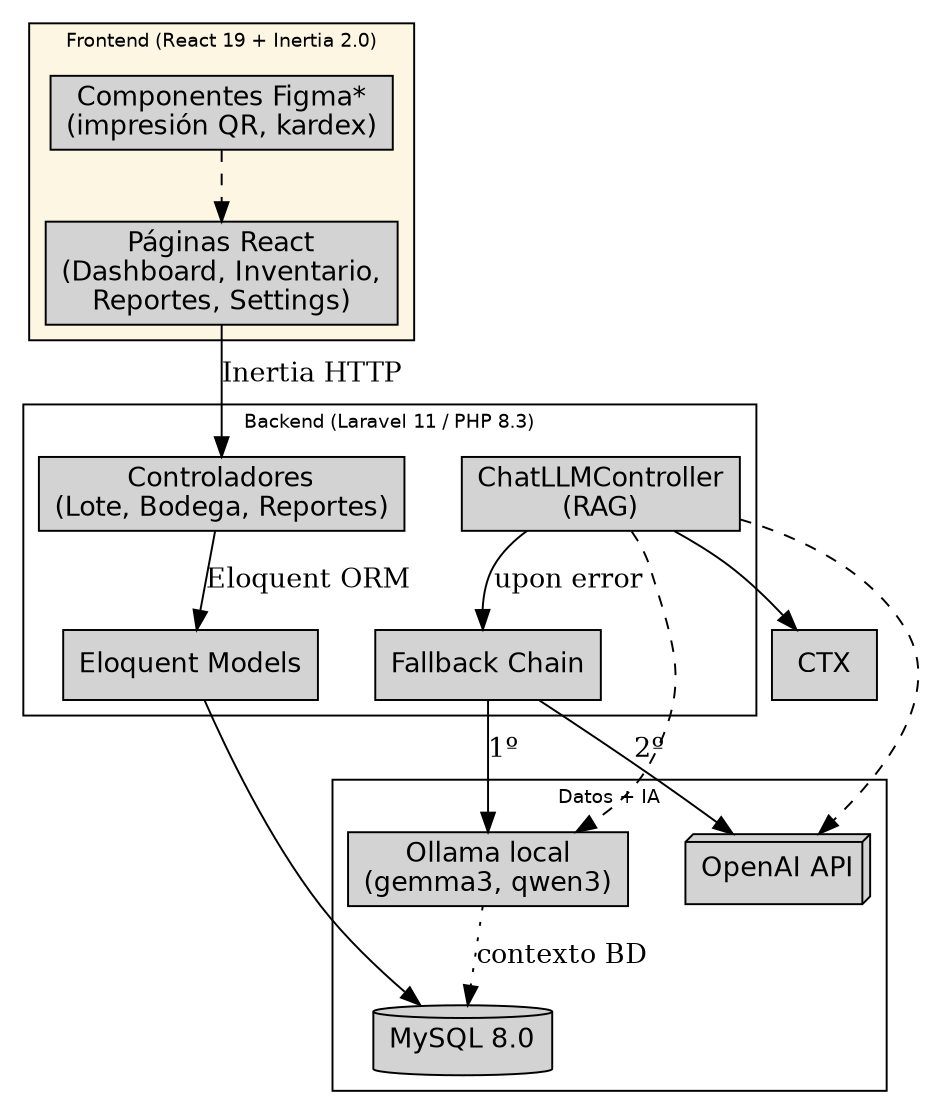
\includegraphics[width=15cm]{Anexos/Imagenes/DiagramaComponentes.png}
	\caption{Diagrama de componentes del sistema Pymetory. Muestra la organización modular en cuatro capas: frontend React, backend Laravel con sus controladores y middlewares, persistencia MySQL con 12 tablas, y el módulo de inteligencia artificial con el RAG Context Builder que conecta la base de datos con OpenAI y Ollama.}
	\label{fig:componentes}
\end{figure}

\subsection*{Diagrama de Despliegue}

\begin{figure}[H]
	\centering
	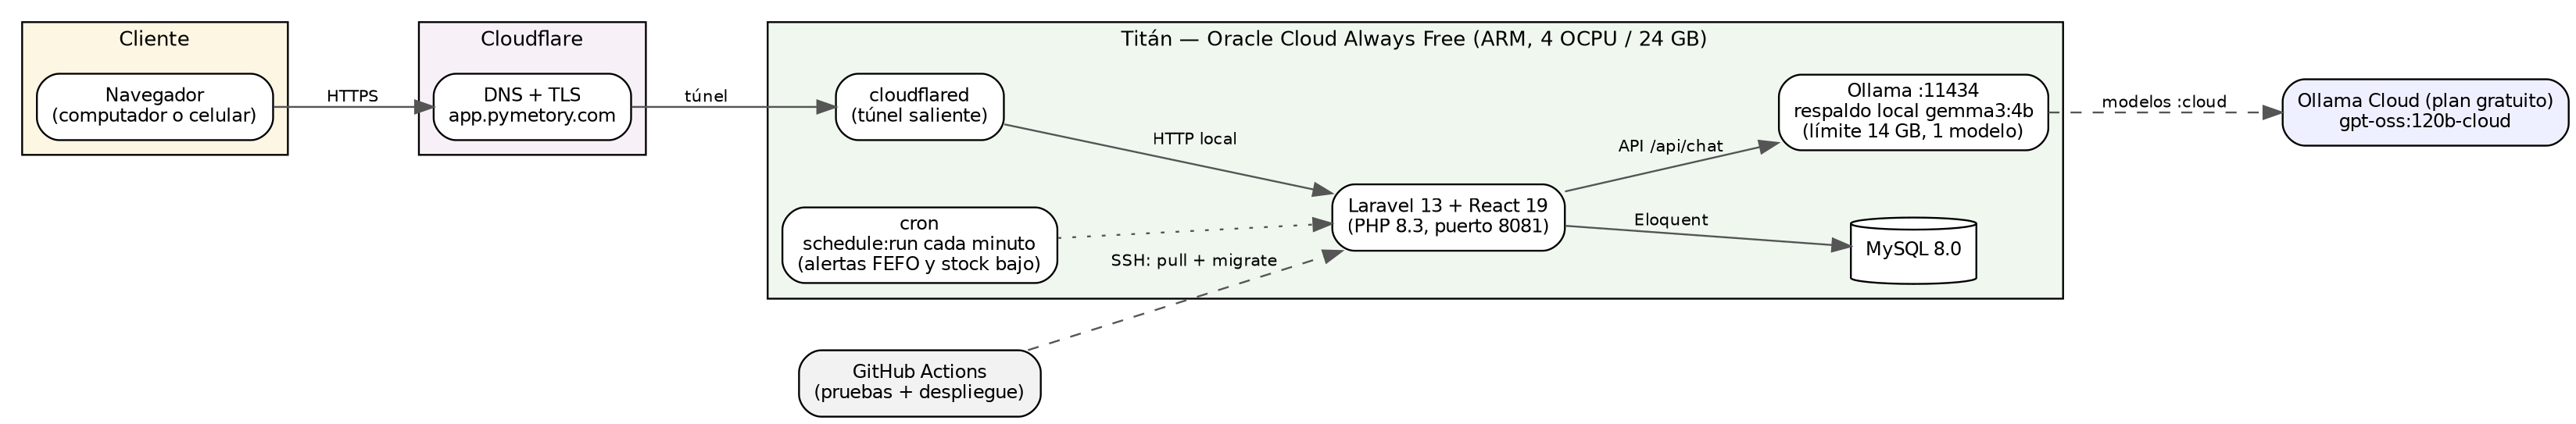
\includegraphics[width=15cm]{Anexos/Imagenes/DiagramaDespliegue.png}
	\caption{Diagrama de despliegue de la infraestructura del sistema. Describe la distribución física: el cliente accede vía navegador por HTTPS, Nginx actúa como proxy inverso, PHP-FPM ejecuta Laravel, MySQL gestiona la base de datos, y el módulo de IA puede usar Ollama local o la API de OpenAI como alternativa de respaldo.}
	\label{fig:despliegue}
\end{figure}

\subsection*{Diagrama de Clases Simplificado}

\begin{figure}[H]
	\centering
	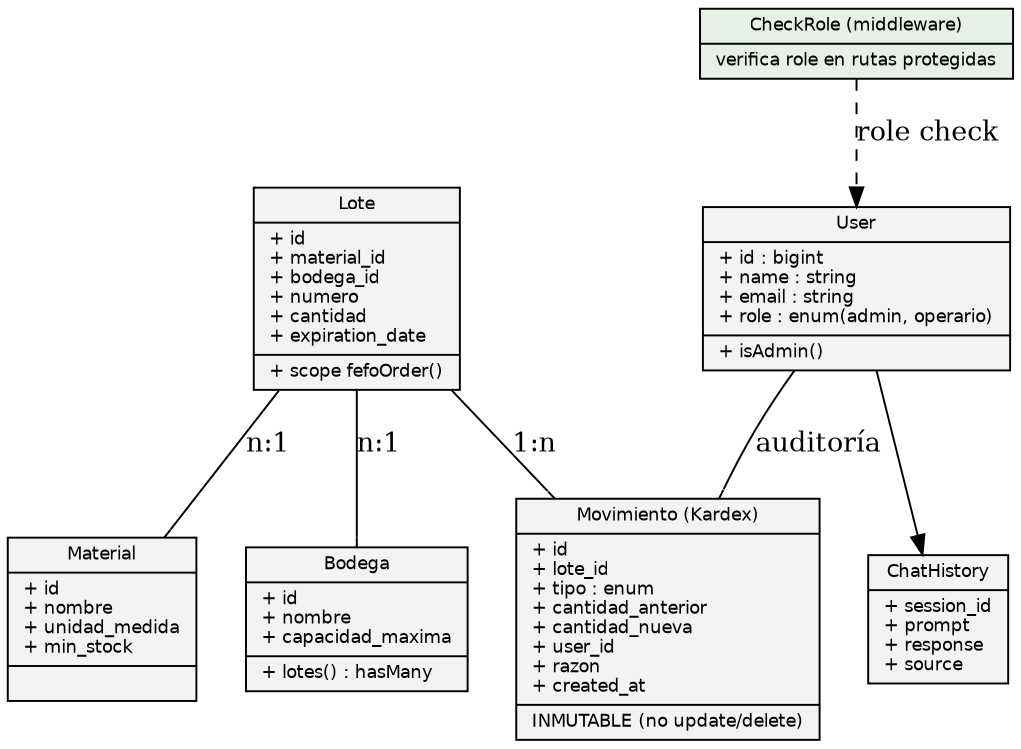
\includegraphics[width=14cm]{Anexos/Imagenes/DiagramaClases.png}
	\caption{Diagrama de clases simplificado con las cinco entidades principales del sistema: User, Bodega, Material, Lote (entidad central FEFO) y Movimiento (Kardex inmutable). Se incluye también ChatHistory para la persistencia de consultas al módulo RAG.}
	\label{fig:clases}
\end{figure}
